\chapter{Contact Planの臨時更新の惑星内への限定的な伝播の提案}
\label{chap:suggestion}
本章では、前章でContact Planの臨時更新時に述べた課題に対して、
その解決策が満たすべき要件について整理し、
Contact Planの臨時更新の際の情報拡散を惑星内に限定することを提案する。
Contact Planの臨時更新の目的は、DTNの各ノードがその時点における
ネットワークのより正確なトポロジー情報を得て、最適な経路を選択できるようにすることである。
DTNのどこかでリンク障害が起きた場合、Contact Planを



\section{Contact Planの臨時更新における要件}
ここでは、Contact Planの臨時更新において満たされるべき要件を整理する。
\subsection{要件1: 臨時更新による経路収束までに要する時間の短縮}
\subsection{要件2: リンク障害による配送遅延増加に対する臨時更新の効果}
ここでは、Contact Planの臨時更新において満たされるべき要件として、
そもそもの目的である実態とかけ離れた状態でCGRを続けることを回避し遅延を抑制すると言う目標にたいして、
情報伝搬範囲を限定することで本提案がそのメリットを損なわないかが重要であるということを述べる。




% \begin{figure}[tbh]
%     \centering
%     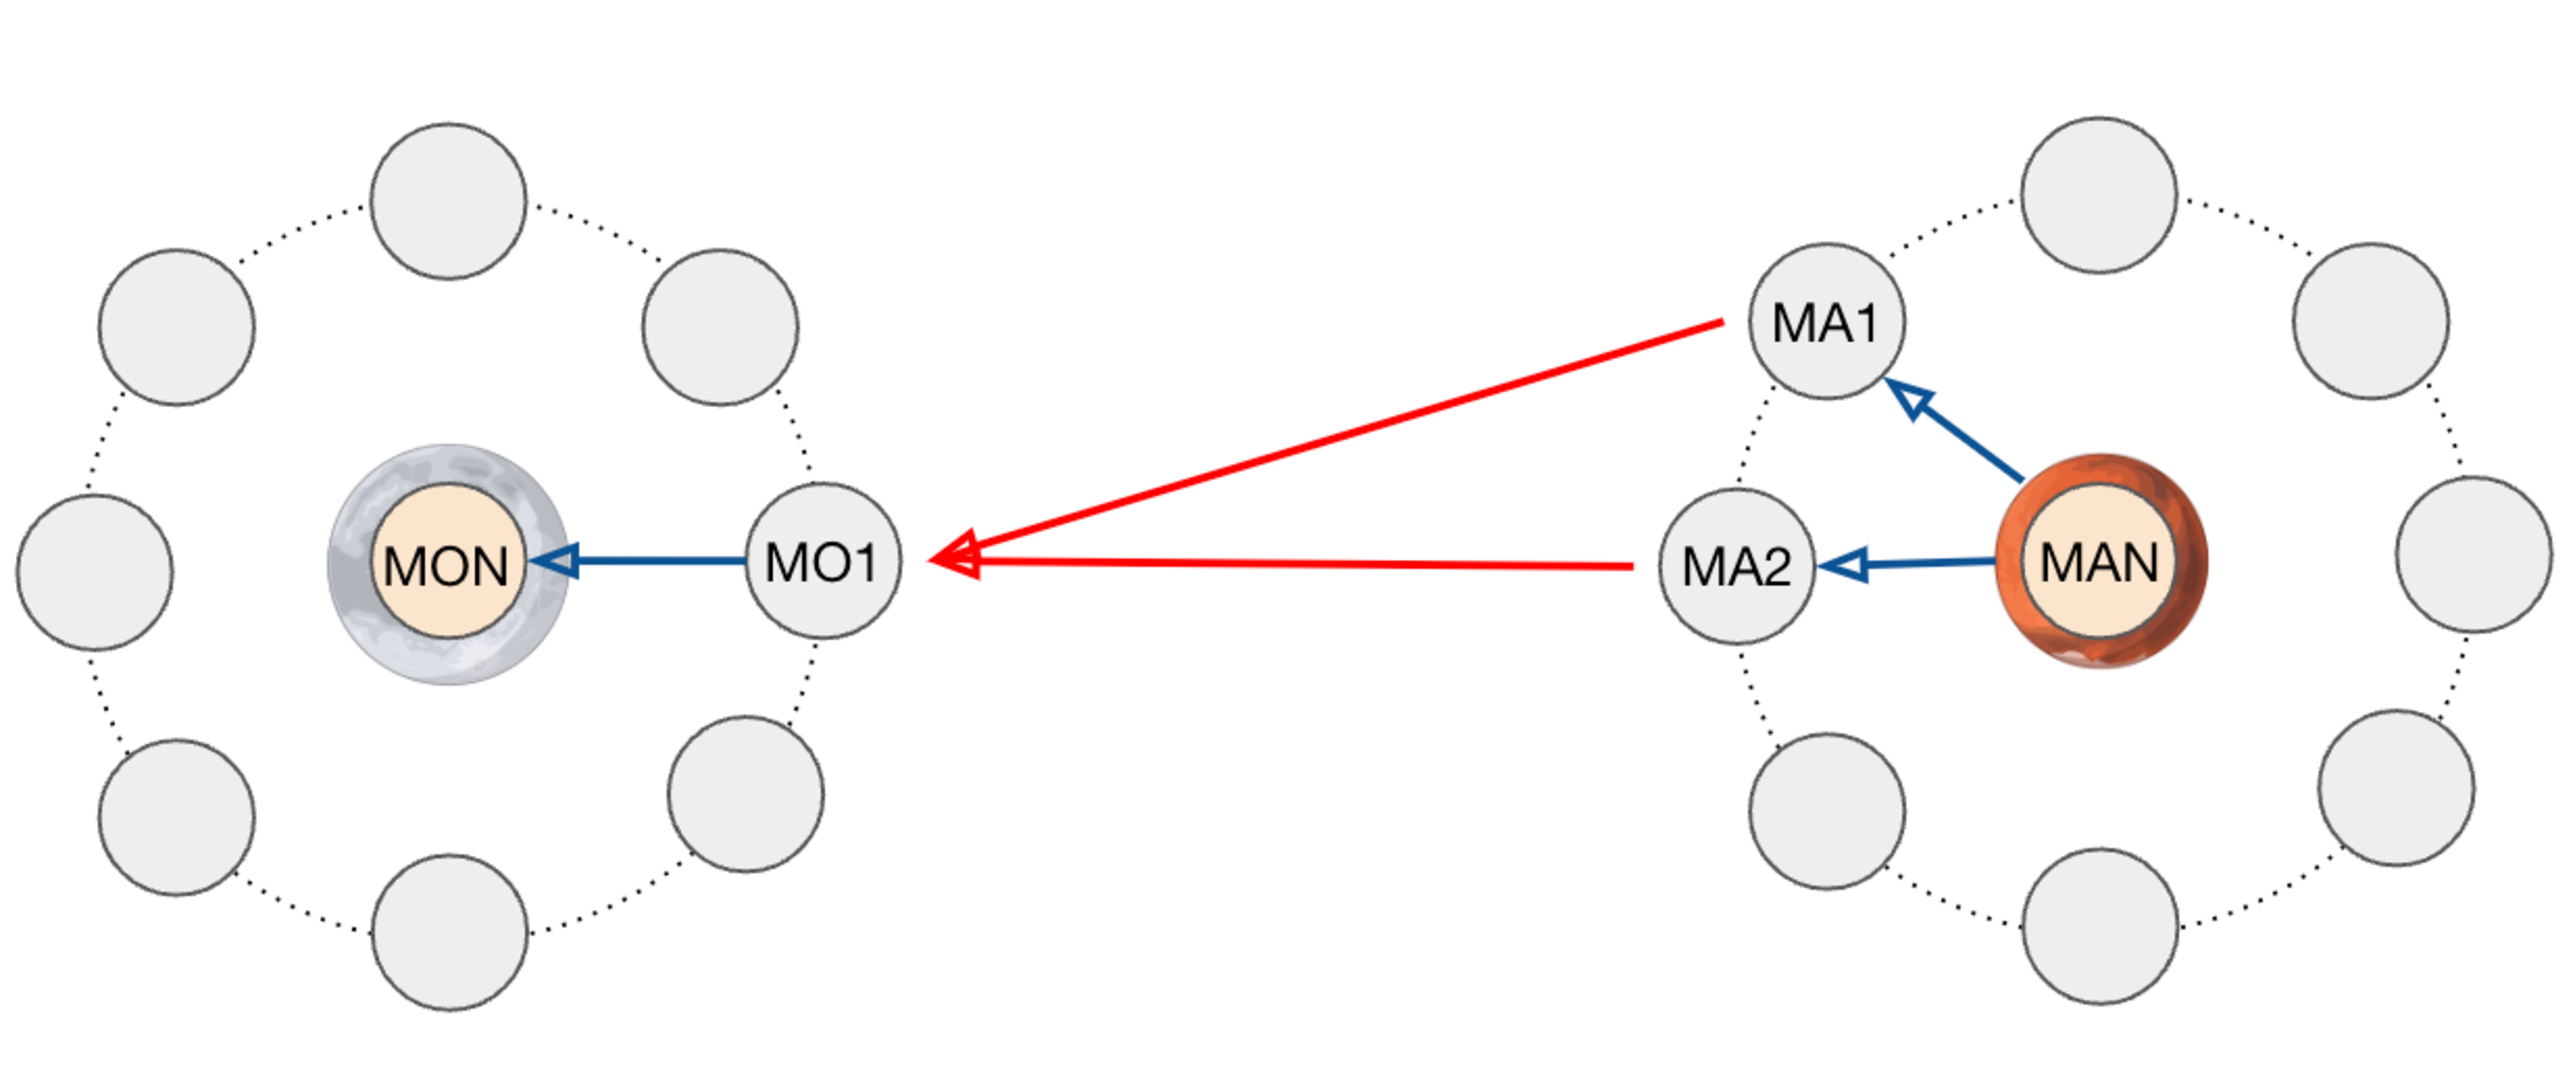
\includegraphics[width=0.7\textheight]{img/ipn_topology.pdf}
%     \caption{2040年代以降のIPNのトポロジー}
%     \label{fig:dtnprotocolstack}
%     \begin{minipage}{\textwidth}
%         \raggedright
%        2040年代以降、IPNは火星にも拡大し、地球・月・火星の3天体間でのIPNが形成される可能性が想定できる。
%     \end{minipage}
% \end{figure}

\section{要件に対する先行手法と本研究の提案手法との比較}
先行研究と本研究の提案手法の比較を行う。
